\documentclass[letterpaper,11pt,twoside,headsepline,bibliography=totoc,index=totoc]{scrbook}
\usepackage{graphicx} % Required for inserting images
\graphicspath{ {./images/} }
% math typesetting packages
\usepackage{amssymb}
\usepackage{amsmath}
\usepackage{amsthm}
\usepackage{mathrsfs}
\usepackage{libertine} % for better paper legibility, easier on the eyes too
\usepackage[T1]{fontenc}
\usepackage[utf8]{inputenc} % for ensuring TeX file(s) are read properly
\usepackage{empheq} % for boxes around equations
\usepackage{framed} % for boxes around text
\usepackage[intoc]{nomencl}
\usepackage{makeidx} % for creating indexes
\usepackage{siunitx} % for typsetting units
\usepackage{xcolor}
\usepackage[bookmarks=true,colorlinks=true, linkcolor=black, urlcolor=violet]{hyperref} % for URLs
\urlstyle{sf} % use sans-serif rather than monospace font for URLs
\usepackage{xpatch}
\usepackage{booktabs} % for tables
\usepackage{microtype} % for nice typography

% ----- CUSTOM COMMANDS ----
% define a new command that adds the URL of a web link at the same time for better experience on print media
\newcommand{\weburl}[1]{\url{#1} \footnote{See website: #1}}
% note: to be used as \webtextlink{link text}{https://somewebsite.com/}. This may lead to errors about "missing
% $ tag inserted", ignore those errors.
\newcommand{\webtextlink}[2]{\href{#2}{#1} \footnote{See website: \url{#2}}}

% Patch page to have underlined chapter titles
% see https://sourceforge.net/p/koma-script/wiki-en/HowTo_ChapterWithLines/
\xapptocmd{\chapterheadstartvskip}{%
  {%
    \setlength{\parskip}{0pt}%
    \setlength{\parfillskip}{0pt plus 1fil}%
    \noindent\rule[.3\baselineskip]{\linewidth}{1pt}\par
  }\nobreak
}{%
  \typeout{Horizontal line before chapter heading added.}%
}{%
  \errmessage{Failed to patch \string\chapterheadstartvskip}%
}%
\xpretocmd{\chapterheadendvskip}{%
  {%
    \setlength{\parskip}{0pt}%
    \setlength{\parfillskip}{0pt plus 1fil}%
    \noindent\rule[-.3\baselineskip]{\linewidth}{1pt}\par
  }\nobreak
}{%
  \typeout{Horizontal line after chapter heading added.}%
}{%
  \errmessage{Failed to patch \string\chapterheadendvskip}%
}%
% end patch

\usepackage[font=small,labelfont=bf]{caption} % for figures/image captions
\usepackage[labelfont=bf]{caption} % figure names/numbers bolded
\usepackage{cinzel}

\makeindex
\makenomenclature

\begin{document}

\title{\normalfont \uppercase{\cinzel{A Learner's Guide to Advanced Theoretical Physics}}}
\subtitle{\small A rigorous self-paced guide to Special and General Relativity, Particle Physics, String Theory, and Quantum Gravity}
\author{\small \sc{Jacky Song and Alex Weiss}}
\date{\normalfont \small{February, 2025}}
% \pagestyle{empty}

\lowertitleback{We dedicate this work to the public domain. We make this dedication for the benefit of the public at large and to the detriment of our heirs and successors. We intend this
dedication to be an overt act of relinquishment in perpetuity of all present and future rights to this work under copyright law.\\\\Jacky Song, Alex Weiss, 2025}

\maketitle



\chapter{Preface}

Welcome! This is a self-learning guide for all readers that want to venture beyond an introductory physics course. In this book, we delve into advanced quantum mechanics and relativity, and don't shy away from the details; we cover the Standard Model \index{Standard Model}, Special Relativity and General Relativity, and the most exciting developments in making a unified theory that bridges General Relativity and the Standard Model. Additionally, we will also spend some time looking into \textit{non-relativistic} quantum field theories, which are very similar to relativistic quantum field theories that form the basis of the Standard Model, except applied to condensed-matter physics and photonics. This guide is mostly targeted for advanced physics undergraduates students, but is written to be accessible enough to be readable by anyone who is curious and wants a challenge.

But, the skeptical reader may ask, why care about theoretical physics? The answer is that basic science, such as research into theoretical physics, is \emph{crucial} to furthering our understanding of science, because it is the bedrock on which all other physics is built upon. The current "Big 2" theories of theoretical physics, General Relativity (GR) \index{General Relativity} and the Standard Model \index{Standard Model}, are both hugely-successful theories, but as of the present moment, attempts to unify the two theories have failed. Thus, working on the problems within each of the theories, as well as their (hopeful) unification, is also (well, subjectively) an interesting intellectual challenge.

We attempt to keep the mathematical prerequisites for this book to the minimum: only some multivariable calculus and some knowledge of vectors and matrices. If these topics are unfamiliar, we highly recommend reading \webtextlink{the free online lecture notes by Professor Paul Dawkins}{https://tutorial.math.lamar.edu/} at Lamar University. We will explain any other mathematics as necessary while we progress through the book.

Our greatest satisfaction is to make the concepts of theoretical physics as clear and accessible as we can. We hope you enjoy this book as much as we have enjoyed writing it.

\tableofcontents
\mainmatter

% respective chapters are in separate files

\chapter{Classical field theory}

Before we get started with either General Relativity or the quantum field theories of the Standard Model, we must look at their shared fundamental structure in \emph{classical field theory}. A classical field theory describes a \emph{field}, which can be thought of as a physical quantity that fills all of space and allows interactions between particles to propagate between each other, leading to what we perceive as "force".

The nebulous idea of a field can be more easily quantified by considering the following example: you stand in a room that has varying temperature. The temperature changes depending on where you are in the room (a physicist would call that \emph{position dependence}), and the temperature also changes over time (in the language of physics, \emph{time dependence}). Thus, if we let $\vec x = \langle x, y, z\rangle$ denote the position in the room and $t$ denote the time, we can write the temperature field, represented as $\phi$, with:

\begin{equation}
\phi(\vec x, t)
\end{equation}

Our modern formulation of classical field theory is that of the \textbf{Lagrangian and Hamiltonian formulation} of classical fields. Such a formulation begins by describing a field in terms of a specific function of the field, called a \textbf{Lagrangian} \index{Lagrangian}, and written as $\mathscr{L}(\phi, \vec x, t)$, where, again, $\phi$ is a function of $\vec x$ and $t$, that is, position and time. (Technically speaking, the more accurate term for fields is to use the term \emph{Lagrangian density}, but we will use an abuse of terminology and simply call the Lagrangian density "the Lagrangian".)

The precise form of the Lagrangian depends highly on which exact field we are studying. But if we want our theories to "make sense" in the physical world, it must satisfy the following constraints:

\begin{enumerate}
    \item Any derivatives of the field that appear in the Lagrangian can be at most \emph{first derivatives}. That is, we can have $\dfrac{\partial \phi}{\partial x}$ or $(\nabla \phi)^2$ as terms in the Lagrangian, but \textbf{not} $\nabla^2 \phi$ as that would be second-order. This is because we do not observe physical fields satisfying partial differential equations (PDEs) \index{Partial Differential Equation} \index{PDE} that include anything above a second-order derivative, and the process we will soon see to determine the PDEs of the fields always raises the order of the derivatives by one.
    \item It must be a function of \emph{individual positions} in space. Thus, the Lagrangian cannot have a term that depends on two positions $\vec x_1, \vec x_2$. This ensures that the field does not violate \emph{locality} (the fact that information propagates at a finite speed and, therefore, information transfer cannot be instantaneous).
    \item It must be scalar-valued and have units of \emph{energy}, and we will see why soon.
\end{enumerate}

There are further restrictions on the specific form of the Lagrangian of a field based on the specific \textbf{symmetries} that we want the Lagrangian (and thus our theory) to obey. For instance, if we want our theory to have \emph{translational symmetry} (symmetric in position), then the Lagrangian \textbf{cannot} contain any terms that would lead to $\mathscr{L}(\phi(\vec x + \vec \epsilon), \vec x + \vec \epsilon, t) \neq \mathscr{L}(\phi(\vec x, \vec t))$, where $\vec \epsilon$ is some shift in position. We may impose further restrictions by requiring, for instance, that the Lagrangian respects \textbf{rotational symmetry} or symmetry upon "flipping" the field (which is the transformation $\phi(\vec x, t) \to \phi(-\vec x, t)$). These symmetries are desirable because a famous theorem known as \textbf{Noether's theorem} says that certain symmetries lead to \emph{conservation laws}, such as the conservation of energy, momentum, and charge, which are fundamental laws of nature. We will also encounter a specific type of symmetry later on called \textbf{Lorentz symmetry} that imposes even stricter conditions on the form the Lagrangian can take. In practice, the combination of symmetries may often be so restrictive that there are only a few possibilities for a field's Lagrangian that can satisfy all the symmetries. But there is no absolute rule for finding the right Lagrangian; even though we can often narrow down the Lagrangian into a much simpler form, the specific Lagrangian that "wins out" in the end is the one that leads to a theory that makes successful predictions, verified by experiments. Physics, is ultimately an \emph{empirical science}, and the source of truth within theoretical physics, just like all other branches of physics, is \emph{consistency with observation}.

\section{The Principle of Stationary Action}

Upon defining a Lagrangian, we can then write out a quantity known as the \textbf{action}. The action $S$ is defined as:

\begin{equation}
S = \int \limits_\text{space+time} \mathscr{L}(\phi(\vec x, t), \vec x, t)\, d^4 x
\end{equation}

Where $d^4 x = dx\, dy\, dz\, dt$, and the integral is conducted over all space and all times. Why define this quantity? Because it turns out that the correct partial differential equation to describe the field $\phi(\vec x, t)$ is the one that makes the action \emph{stationary}. Stationary is a concept that comes from calculus; for the action, it means that rate of change of the action with respect to change in $\phi$ must be zero, which we write as:

\begin{equation}
\delta S = 0
\end{equation}

This requirement for the action being stationary is (unsurprisingly) called the \textbf{Principle of Stationary Action}. It is also sometimes called the Principle of \emph{Least} Action, although the action may not always be a minimum, so that alternate term can be misleading. It turns out (we will not show here as it is a rather involved derivation) that this means that the Lagrangian must satisfy the following partial differential equation:

\begin{equation}
\frac{\partial \mathscr{L}}{\partial \phi} - \partial_\mu \left(\frac{\partial \mathscr{L}}{\partial (\partial_\mu \phi)}\right) = 0
\end{equation}

This partial differential equation is called the \textbf{Euler-Lagrange Equation} for fields \index{Euler-Lagrange Equation} and always gives the correct PDE for the field. We refer to this PDE as the \textbf{equation of motion} of the field, as it describes how the field evolves through time and changes in space. Solving the PDE (with suitable boundary conditions) allows us to find the field as a function of position and time.

Rather incredibly, the basic mathematics and structure of classical theories of fields carry over even to domains where classical mechanics no longer holds - including the relativistic and quantum domains. This is why it remains an important area of study over 200 years since its inception.
\chapter{Introduction to Special and General Relativity}

General Relativity\index{General Relativity} is doubtlessly one of the most beautiful theories of physics ever devised. It is, sadly, also quite complicated. I hope this attempt to explain it, going step-by-step through all the little details, will hopefully clear up some of the confusion for first-time learners, while still doing the subject justice.
\chapter{Introduction to Quantum Field Theory}

Quantum field theory (QFT) \index{Quantum Field Theory} is our most accurate description of the universe at the microscopic scale. The \textbf{Standard Model}, a comprehensive quantum field theory, is the backbone of modern physics, and has been tested to extreme precision. Despite this, quantum field theory has a reputation for not being very accessible, in part because of its scary-long Lagrangians and incredibly formidable integrals. But we will hopefully show that it is not as formidable as it may seem --- in fact, it can be quite satisfying for the curious reader!

\section{The motivation for quantum field theory}

All matter in the universe is quantum in nature. Quantum mechanics governs the behavior of all matter, and at an introductory and intermediate level, the dynamics of quantum systems is typically solved with the Schrödinger equation:

\begin{equation}
i\hbar \dfrac{\partial}{\partial t} \Psi(\mathbf{r}, t) = \left(-\dfrac{\hbar^2}{2m} \nabla^2 + V(\mathbf{r})\right) \Psi(x, t)
\end{equation}

However, relativistic quantum field theory is a far more accurate theory of quantum mechanics than the Schrödinger equation. In fact, while we may use approximations like (semi-)classical theory and nonrelativistic or single-particle quantum mechanics, quantum field theory, and specifically the Standard Model, offers the best and most accurate results. 

That is to say, any quantum system may be solved for by the Schrödinger equation, but doing the same calculations with quantum field theory offers results with unparalleled precision. Predictions of the \webtextlink{magnetic moment of electrons}{https://en.wikipedia.org/wiki/Magnetic_moment}, \webtextlink{energy levels of the hydrogen atom}{https://en.wikipedia.org/wiki/Lamb_shift}, a variety of \webtextlink{previously-unknown elementary particles}{https://physics.info/standard/}, and the \webtextlink{Rydberg constant}{https://en.wikipedia.org/wiki/Rydberg_constant} made through quantum field theory have been experimentally tested and confirmed very well.

These are not meaningless predictions either; our understanding of the emission and absorption of light, of the subatomic origins of magnetism, and even our standard of time in the \webtextlink{definition of a second}{https://en.wikipedia.org/wiki/Second} are based on these predictions. In turn, numerous scientific experiments, material science, laser technology, and electronics depend on applying these predictions, without which they would likely not progress to how they are today.

Quantum field theory is a very rewarding, if difficult, theory to learn. But given its place as the best theory of matter physics ever devised - learning it is worth it.

\section{Common beginner misconceptions}

Quantum field theory has a lot of confusing parts, and so it's best to understand these before going too far into it:

- Quantum field theory is \textbf{not} string theory, they are distinct theories that share some similarities but are not extensions of each other
- Even though it is mostly used in very specific cases due to its complexity, quantum field theory is a \textbf{more fundamental theory} than classical field theory and classical field theory is its limiting case
- The interpretations of PDEs (equations of motion) is \textbf{different} in quantum field theory as compared to quantum mechanics; quantum field theory PDEs, even complex-valued ones, have none of the probability interpretation of the Schrödinger equation

\section{Canonical quantization}

Start with a suitable classical Lagrangian of the fields to be studied. If you don't know one and can't copy one from a book or ask someone, then just propose one (i.e. make an educated guess). For instance, if you were studying the electron field, then maybe you would want to use this Lagrangian:

\begin{equation}
\mathscr{L} = \overline \psi (i \gamma^\mu \partial_\mu - m) \psi
\end{equation}

Plug that Lagrangian into Euler-Lagrange equations, here with $\varphi = \psi(x^\nu)$:

\begin{equation}
\frac{\partial \mathscr{L}}{\partial \varphi} - D_\mu \left(\frac{\partial \mathscr{L}}{\partial (\partial_\mu \varphi)}\right) = 0
\end{equation}

Then you get the equations of motion of the field (PDEs). E.g. for Higgs field this is the complex-valued Klein-Gordon equation, for quarks and electrons this is the Dirac equation, for photons this is Maxwell's equations. In our case this is the Dirac equation, which describes all matter fields (i.e. those of electrons and quarks, which make up all atoms):

\begin{equation}
(i \gamma^\mu D_\mu - m) \psi = 0
\end{equation}

The associated quantum fields obey the operator equations of motion, which are the \textbf{same} as the PDE equations of motion but operator-valued. For the electron field this is:

\begin{equation}
(i \gamma^\mu D_\mu - m) \hat \psi = 0
\end{equation}

Where we just made the change $\psi \to \hat \psi$ to get an operator-valued equation of motion. Meanwhile, the electromagnetic field $A^\mu$ satisfies Maxwell's equations:

\begin{align*}
\partial^\nu \partial_\nu A^\mu = \mu_0 J^\mu
\end{align*}

It is important to note that the Dirac equation takes on a special interpretation in QFT. It in fact becomes a \emph{classical equation of motion} of a Dirac field $\psi$, rather than a wavefunction. The complex-valued $\psi$ can be thought of as a combination of two real fields $\psi_\alpha$ and $\psi_\beta$ where $\psi = \psi_\alpha + i \psi_\beta$. The physical interpretation of the Dirac field is that it is a field of electrons within space, where the 4-current produced by the electrons is $J^\mu = \psi \gamma^\mu \bar \psi$.

You solve for those operator equations of motion by first solving the PDE equation of motion for the field. Then from there you can promote the field to an operator. One could solve the operator equation of motion directly, but that approach can lead to substantial confusion; an operator may not be commutative and the partial derivative of an operator may not be so simple to find. It is far easier to just solve the PDE equation of motion and then promote the solution to an operator rather than directly trying to solve the operator equation of motion. For quantum electrodynamics the field operator is:

\begin{align*}
\hat A^\mu(x) = \int \frac{d^3k}{(2\pi)^3} \sum_{\lambda=1,2} \left( \epsilon^\mu(\mathbf{k}, \lambda) a(\mathbf{k}, \lambda) e^{-ik \cdot x} + \epsilon^{\mu *}(\mathbf{k}, \lambda) a^\dagger(\mathbf{k}, \lambda) e^{ik \cdot x} \right)
\end{align*}

Where $a, a^\dagger$ are creation and annihilation operators, more on that later. 

\begin{framed}
\textbf{Note:} Remember that this is an \emph{operator}, not a state or
function.
\end{framed}

After you get the field operator, you then want to construct the series of (eigen)states of the field, from which you can calculate the probability amplitudes of processes. To do so, you find the field Hamiltonian, which has the same expression as the Hamiltonian density in classical field theory, except substituting the classical field with the field operator. For quantum electrodynamics this is:

\begin{equation}
\hat{\mathcal{H}}=\sum _{\mathbf {k} ,\mu }\hbar \omega \left({a^{\dagger }}^{(\mu )}(\mathbf {k} )a^{(\mu )}(\mathbf {k} )+{\frac {1}{2}}\right)
\end{equation}

Now you want to find the eigenstates of the Hamiltonian (which are the possible states of the field), and specifically, you want to find the ground state. Analogous to the quantum harmonic oscillator's ladder operators, you then find the annihilation (lowering) and creation (raising) operators by commutation relations. Then, by imposing the condition that the annihilation operator applied to the ground state creates the zero (vacuum) state. In the case of quantum electrodynamics the ground state is given by $|0 \rangle$ where:

\begin{equation}
\hat a (\mathbf{k}, \lambda)| 0 \rangle = 0
\end{equation}

The raising operator can then be used to find all the excited states of the quantum field, just like the quantum harmonic oscillator. Then, we can calculate energy eigenvalues and expectation values associated with each energy eigenstate, and we can calculate the probability of the fields going from one state to another state, which is fundamental to the study of scattering processes. For scattering specifically, we calculate an \emph{S-matrix} $\hat S$ defined as the operator that acts on an initial state $|i \rangle$ to produce a final state $|f\rangle$ where the probability amplitude is $C$:

\begin{equation}
C = \langle f | \hat S | i \rangle
\end{equation}

The \emph{S-matrix} is calculated through what is known as a \textbf{Feynman diagram} that represents, graphically, the contributions to the S-matrix integral. For instance, below is the representation of an electron-position annihilation, which produces two photons (in the gamma ray wavelengths):

\begin{figure}[h]
    \centering
    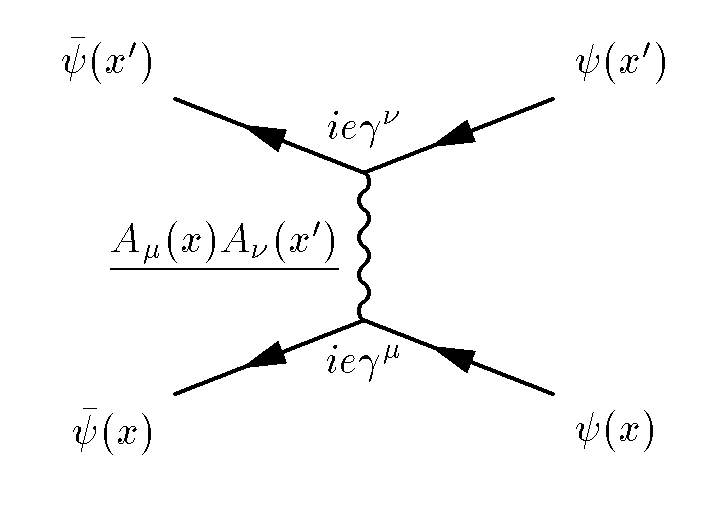
\includegraphics[width=0.5\linewidth]{Feynman-diagram-ee-scattering.png}
    \caption{A Feynman diagram showing the electron-positron annihilation interaction in terms on ingoing and outgoing lines.}
    \label{fig:feynman-scattering}
\end{figure}

The ground state, meanwhile, gives the \textbf{zero-point energy} of the electromagnetic field. It is not possible in quantum mechanics to have a zero energy vacuum state, because that would violate the energy-time uncertainty principle. Thus, the zero-point energy exists even in a vacuum. In quantum electrodynamics, the expression of the zero-point energy is given by:

\begin{equation}
E_0 = \sum_{\lambda = 1, 2} \int \dfrac{d^3 k}{(2\pi)^3} \dfrac{\hbar \omega_\mathbf{k}}{2} - \int \dfrac{d^3 p}{(2\pi)^3} \hbar \omega_\mathbf{p}
\end{equation}

This zero-point energy has important implications for cosmology, primarily because while we understand it perfectly well in terms of quantum field theory, we don't understand it well in terms of cosmology. In addition, it gives rise to many quantum effects such as the \textbf{Casimir effect}, where a force is observed that acts as a negative pressure pulling two plates together, even in vacuum.

\section{Effective field theory}

So you realize immediately when doing QFT for any amount of time that a lot of calculations end up with integrals that are divergent. Sometimes, there are clever ways to evaluate those integrals to end up with a reasonable value, but sometimes, there isn't. When that's the case, we can use something called \emph{effective field theory}.

Effective field theory is the idea that whenever we are trying to apply quantum field theory, we ask ourselves "how precise do we need the results to be?" From there, we can set an upper bound for the theory in terms of the precision required, and remove all the terms that are suppressed by that upper bound.

As a classical analogy, consider the expression of the kinetic energy in classical mechanics. From a quick wikipedia search, the \emph{relativistic} kinetic energy is given by the expression:

\begin{equation}
K = (\gamma - 1) mc^2 = \frac{mc^2}{\sqrt{1 - (v /c)^2}} - mc^2
\end{equation}

Using a Taylor expansion we can write this as:

\begin{equation}
K = \frac{1}{2} mv^2 + \frac{3}{8} m \frac{v^4}{c^2} + \dots
\end{equation}

% the following paragraph will result in an warning due to
% the link, please ignore that warning
But suppose we were interested in scales where $v \ll c$. In this case we can set an upper bound for $v$, what is known in QFT as a \webtextlink{https://en.wikipedia.org/wiki/Cutoff_(physics)}{cutoff}. Then we can ignore the higher-order terms in the expression of kinetic energy, so it simply becomes:

\begin{empheq}[box=\fbox]{equation}
K = \frac{1}{2} mv^2
\end{empheq}

A similar procedure works in QFT. In the perturbative expansion, we ignore higher-order terms.

\section{The non-relativistic and classical limit}

In many situations, we study quantum field theories under non-relativistic conditions (for instance, for quantum optics such as lasers, or for studying the properties of multi-atomic systems such as solids).

Let us show how we are able to recover the Dirac and Schrodinger equations, and in the case of quantum electrodynamics, even Maxwell's classical equations of motion, in the non-relativistic and (in the latter case) classical limit.

\section{Other formulations of quantum field theory}

There are other formulations of quantum field theory that will be covered in the following sections here:

- Lattice grid QFT
- Algebraic QFT
- Topological QFT
- Conformal field theory

\section{Quantum Gravity: An exercise for the reader}

You know how some textbooks like to say "the full solution is left as an exercise to the reader?" Well, let's work out a fun exercise for the reader: quantizing gravity!

For gravity, we start with the Lagrangian for General Relativity \index{General Relativity}:

\begin{equation}
\mathscr{L} = \frac{1}{16 \pi G} R \sqrt{-g} + \mathscr{L}_{SM} \sqrt{-g}
\end{equation}

Solving the Euler-Lagrange equations results in the most general form of the Einstein field equation:

\begin{equation}
G_{\mu \nu} + \Lambda g_{\mu \nu} = 8\pi G T_{\mu \nu (SM)}
\end{equation}

where $T_{\mu \nu (SM)}$ is the stress-energy tensor (mass-energy field) of all the matter content within spacetime. In QFT, the Einstein field equation becomes an operator-valued equation, so we promote all the fields to operators, resulting in:

\begin{equation}
\hat G_{\mu \nu} + \Lambda \hat g_{\mu \nu} = 8\pi G \hat T_{\mu \nu (SM)}
\end{equation}

Up to this point, we have been operating within the realm of known physics. We know the right-hand side of this equation: it is simply the combined stress-energy of the standard model. And we know that the left-hand side must hold true, due to the correspondence principle. But we \emph{don't} know what form the left-hand side must take, that is, what the operators have to be to satisfy this operator equation.

\subsection{Semiclassical quantum gravity}

An example is Hawking radiation...

\section{Computational methods and Lattice QFT}

Analytical calculations have been the mainstay of quantum field theory for many decades, and it makes sense why: the number of mathematical tricks and divergences to remove makes QFT integrals a nightmare for numerical (computational) methods. Despite this, it is possible to do some parts of QFT computationally.
\chapter{Non-relativistic quantum field theory}

As we mentioned at the start of the book, not all quantum field theories are relativistic in nature. Some quantum field theories are \emph{non-relativistic} and describe continuum states of matter or light interacting with matter that do not fall in the high-energy regime. Non-relativistic quantum field theories are used extensively in condensed-matter physics, such as the theories of superconductivity in matter, as well as photonics, such as the theory of lasers and a complete description of the photoelectric effect.

\backmatter
\clearpage

\nomenclature{$c$}{Speed of light in a vacuum, \qty{299792458}{\m\per\s}}
\nomenclature{$h$}{Planck constant}
\nomenclature{$\hbar$}{Reduced Planck constant}
\nomenclature{$e$}{Elementary charge constant}
\nomenclature{\partial_\mu}{Equal to $\dfrac{\partial}{\partial x^\mu}$, partial derivative with respect to the $\mu$-th coordinate}
\nomenclature{\partial^\mu}{Equal to $g^{\mu \nu}\partial_\nu$, where $g^{\mu \nu}$ is the inverse metric; typically speaking, the inverse metric is the Minkowski metric $\eta^{\mu \nu}$}
\nomenclature{\displaystyle \int d^4 x}{Integral over all spacetime; $d^4x$ is shorthand for $dx\,dy\,dz\,dt$}
\nomenclature{\displaystyle \int d^3 x}{Integral over all space; $d^3x$ is shorthand for $dx\,dy\,dz$}
\printnomenclature

\printindex

\end{document}